\section{Sistema embarcado}
A Raspberry Pi é um microcomputador sistema operacional Linux, que foi escolhida para ter o programa embarcado que controla e monitoriza a estufa devido a facilidade de acesso aos seus pinos GPIO para conectar diversos sensores e atuadores, como ela já tem conectividade Wi-Fi, será facilmente facilmente conectada a internet apenas acessando a rede local do usuário e ela já tem autorização pela Anatel, com suas entradas USB, é possível conectar uma câmera USB e utilizá-la para monitorizar a estufa.[1]

Especificações:

\begin{itemize}
	\item Raspberry Pi 3 Model B Anatel
	\item Processador Broadcom BCM2837 64bit ARMv8 Cortex-A53 Quad-Core
	\item Clock 1.2 GHz
	\item Memória RAM: 1GB
	\item Adaptador Wifi 802.11n integrado
	\item Bluetooth 4.1 BLE integrado
	\item Conector de vídeo HDMI
	\item 4 portas USB 2.0
	\item Conector Ethernet
	\item Interface para câmera (CSI)
	\item Interface para display (DSI)
	\item Slot para cartão microSD
	\item Conector de áudio e vídeo
	\item GPIO de 40 pinos
	\item Número de homologação Anatel: 04908-17-10629 
	\item Dimensões: 85 x 56 x 17mm[1]
\end{itemize}

\section{Medição do Nível da Água}

O tipo de medição escolhida foi a descontinua e o Sensor de nível de água eletrônico - ON/OFF – US23. Este sensor de nível é uma chave ON/OFF (Liga/desliga) que muda o estado de aberto para fechado quando a água atinge certo nível e abre quando o nível da água fica abaixo de outro determinado nível. Este sensor pode chavear diretamente cargas de até 10W 220V, como bobinas de contatores ou pequenas lâmpadas de sinalização.

No caso do projeto da estufa, ele irá chavear uma tensão de 3.3 V e corrente de 3.3 mA, garantida por um resistor de 10K$\Omega$. E serão utilizadas duas bóias na seguinte disposição da figura abaixo: [2]

\begin{figure}[H]
	\centering
	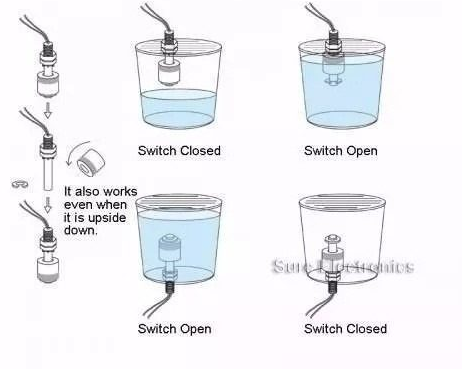
\includegraphics[width=6cm]{figuras/eletronica_1.png}
	\caption{Disposição das Bóias no Reservatório} \label{eletronica_1}
\end{figure}

Uma ao fundo para definir se o nível da água está baixo e um em cima definir o nível de água baixo.  A leitura do estado dos sensores será feita atraves do pino GPIO, onde o estado HIGH (tensão de 3.3V ) indica que o sensor foi ativado e o estado LOW( tensão de 0V) indica que ele está desativado.[2]

Este sensor de nível utiliza um sensor magnético e não mercúrio que seria prejudicial à saúde.[2]

Características:

\begin{itemize}
	\item Comprimento do cabo: 36cm
	\item Máxima potência da carga: 10W
	\item Máxima tensão: 220V DC
	\item Máxima corrente de chaveamento: 0.5A
	\item Máxima corrente de carga: 1A
	\item Resistência do contato: 0.1 $\Omega$
	\item Temperatura de trabalho: -10°C ~ + 60°C
	\item Dimensões da boia: 23mm x 22mm
	\item Comprimento do sensor: 57mm
	\item Diâmetro do eixo: 8mm
	\item Diâmetro da rosca: 9mm
\end{itemize}

\section{Optoacoplador 4N25}

O optoacoplador escolhido foi 4N25, que é contituído por um diodo emissor de luz e um foto transistor bipolar. E funciona como mostrado na figura abaixo:

\begin{figure}[H]
	\centering
	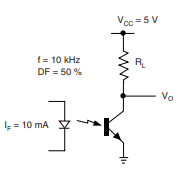
\includegraphics[width=8cm]{figuras/optocoaplador.png}
	\caption{Funcionamento do optoacoplador} \label{optocoaplador}
\end{figure}

A Raspberry irá controlar o LED interno do optoacoplador, quando o LED está aceso o transitor é “ativado” e permite a passagem de corrente através dele. E quando o LED está apagado o trasnsitor fica em situação de corte e não permite a passagem de corrente.

Para o projeto da estufa foi confeccionada uma placa com com 8 optoacopladores, figura abaixo, que serão conectados aos relés que garantirão uma proteção a mais para o circuito.[3]

\begin{figure}[H]
	\centering
	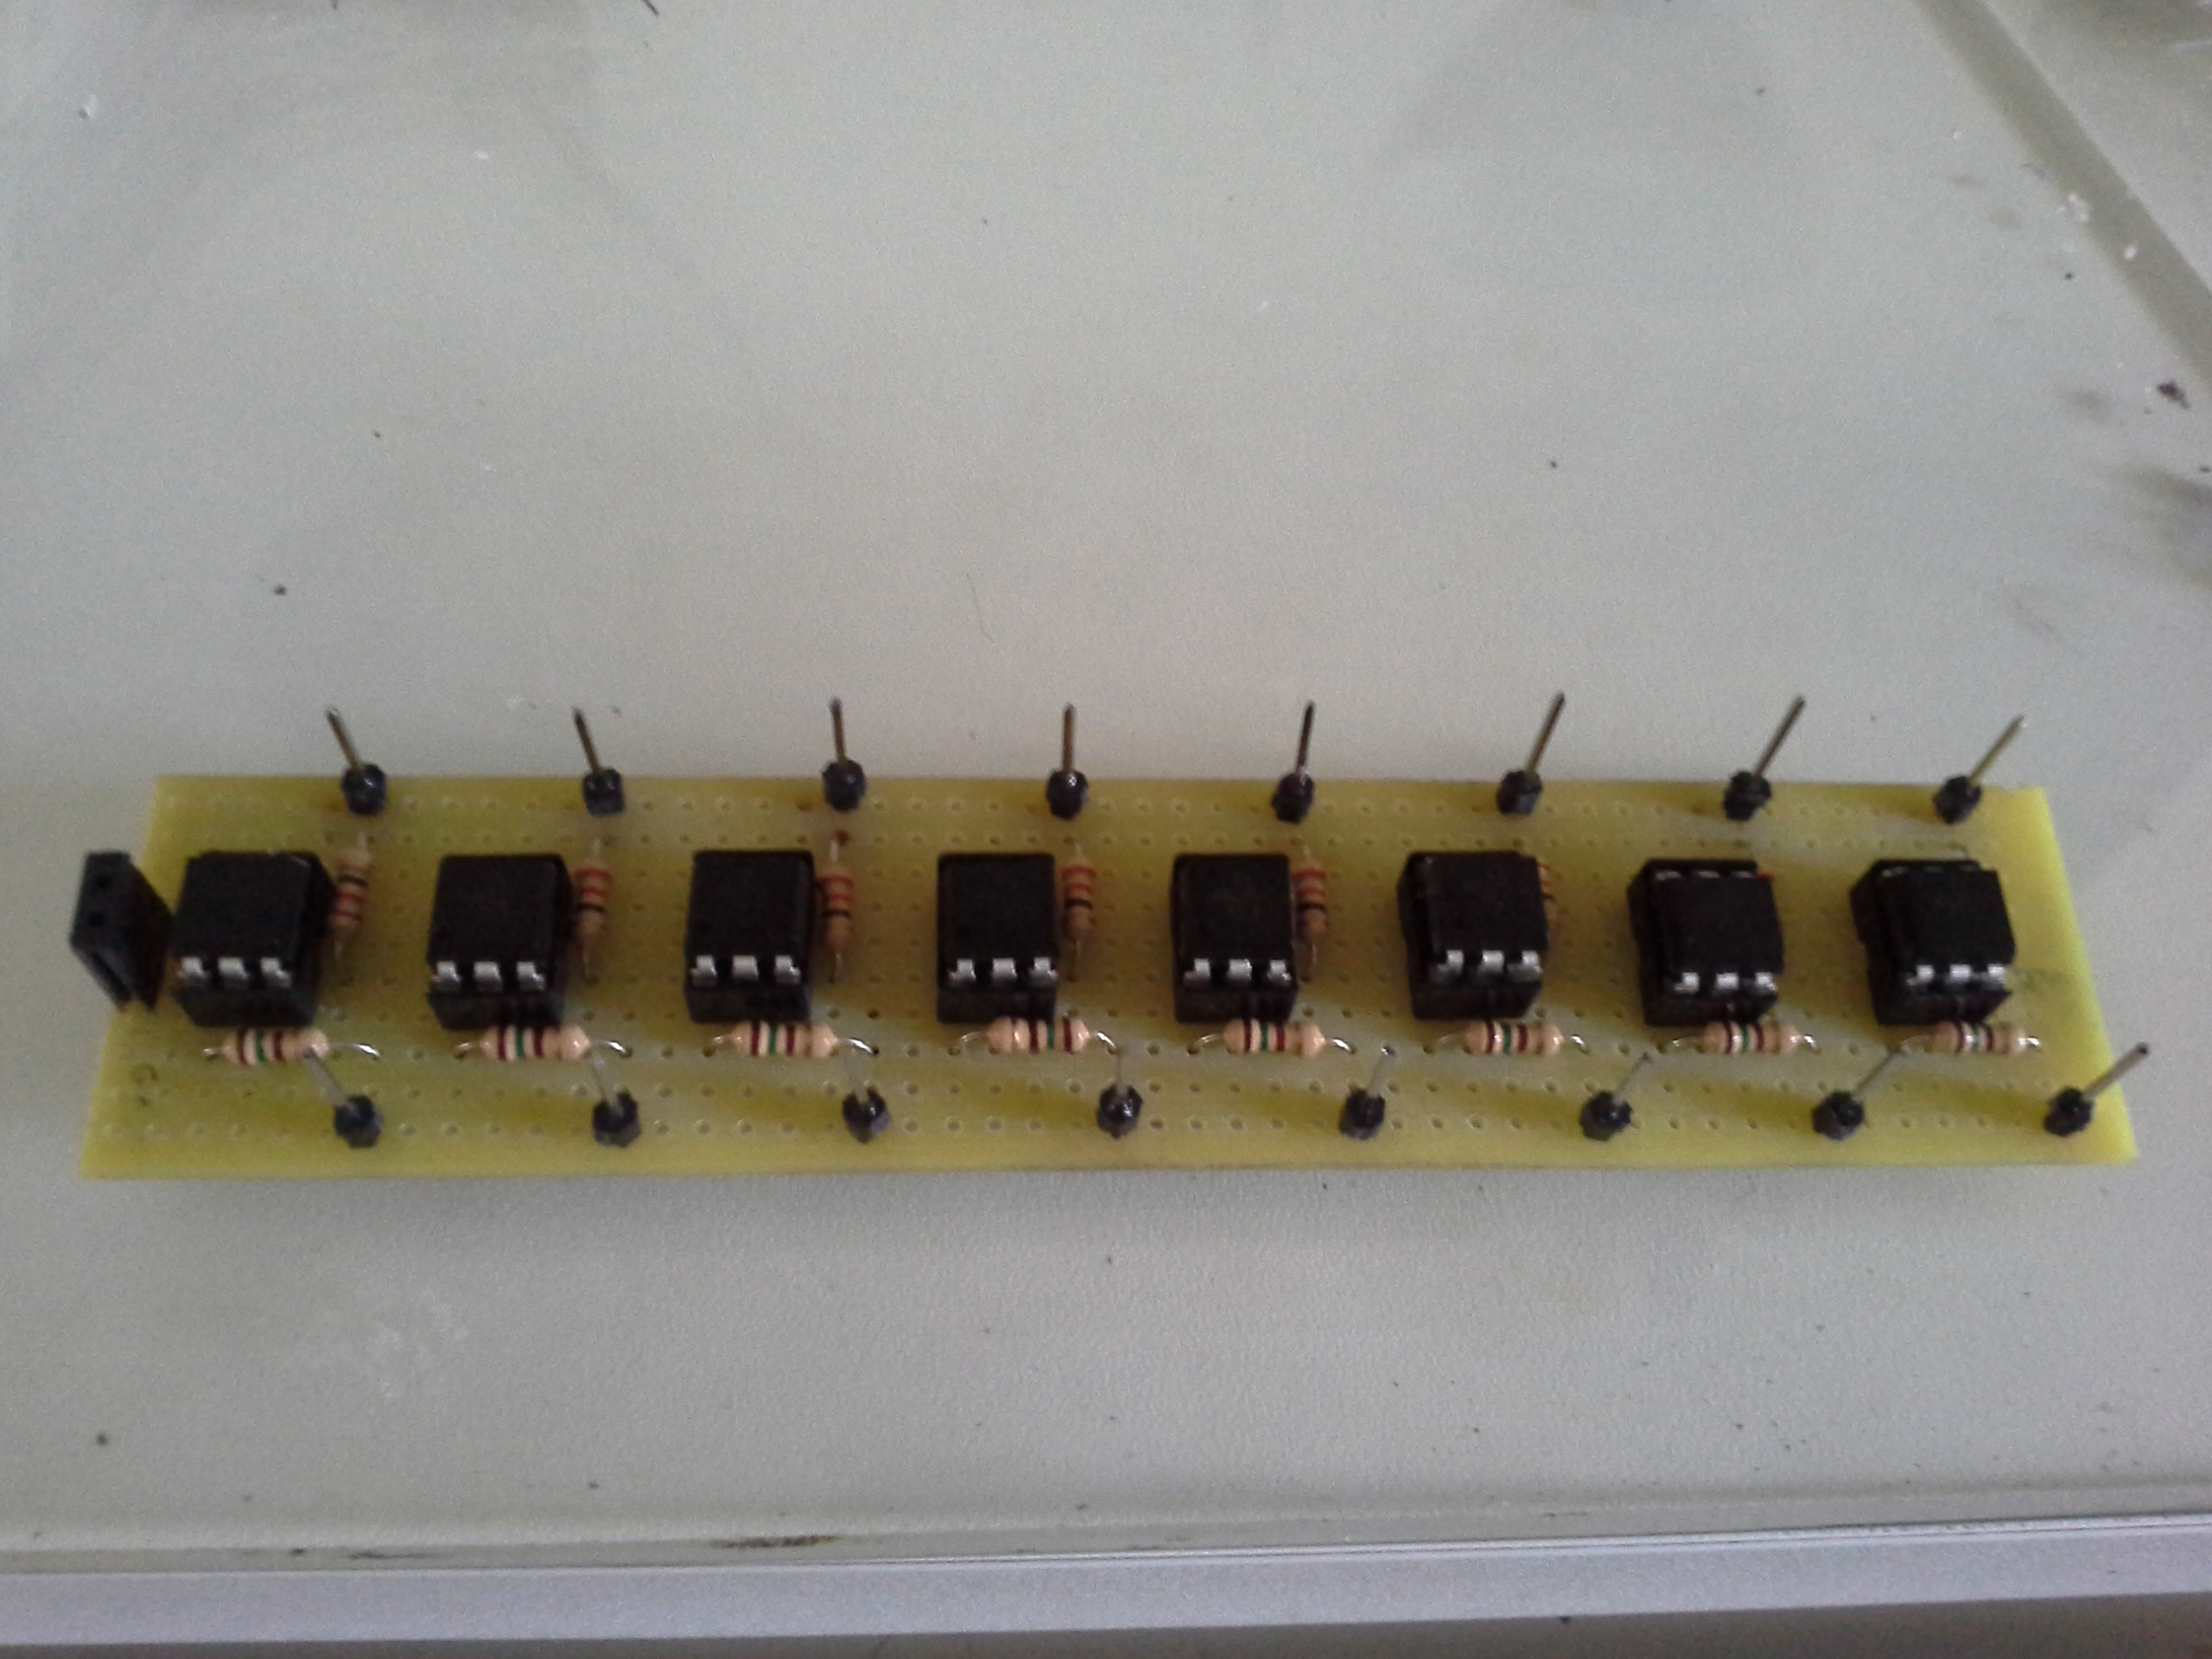
\includegraphics[width=15cm]{figuras/optoacopladores.jpg}
	\caption{Funcionamento do optoacoplador} \label{optoacopladores}
\end{figure}

\section{Relé}

No projeto da estufa os relé serão utilizados para acionar as 3 bombas de água responsáveis pela circulação de água, os coolers de circulação de ar, as válvulas solenóides que controlam a torca de água do reservatório, as lâmpadas da estufa e o compressor de ar do reservatório de água.

Como serão vários dispositivos e consequentemente vários relés, o grupo optou por comprar um módulo relé de 8 canais.[4]

\begin{figure}[H]
	\centering
	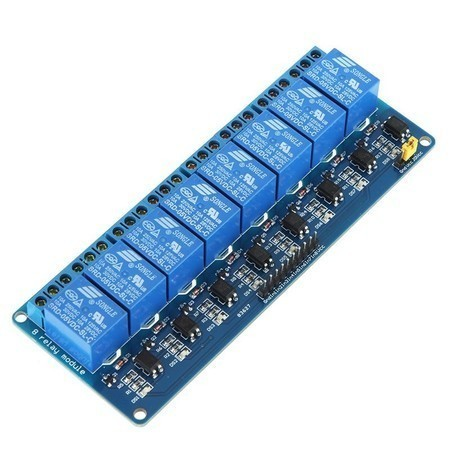
\includegraphics[width=8cm]{figuras/modulo_re.jpg}
	\caption{Módulo Relé de 8 canais} \label{modulo_re}
\end{figure}

Ele será ativado pelo pinos GPIO da Raspberry Pi, que estarão isolados por um optoacoplador.

\section{Conversor analógico para digital}

A Raspberry Pi não possui conversor AD integrado, como alguns microcontroladores, e alguns dos sensores utilizados no projeto precisam de um, pois apresentão seus dados de forma analógica. Para contornar essa dificuldade haviam duas possibilidades, utilizar um microcontrolador com conversor analógico integrado e realizar a comunicação do mesmo com a Raspberry, ou conectar um conversor AD diretamente a Raspberry. A opção escolhida pelo grupo foi a segunda, pelo baixo custo e pela oportunidade de aprender a utilizar um conversor AD pelos membros do grupo de eletrônica.[5]
 
O conversor escolhido foi PCF8591, que é um dispositivo de aquisição de dados CMOS de 8 bits de alimentação única e baixo consumo de energia, com quatro entradas analógicas, uma saída analógica e uma interface de barramento I2C serial. Três pinos de endereço A0, A1 e A2 são usados para programar o endereço de hardware, permitindo o uso de até oito dispositivos conectados ao barramento I2C sem hardware adicional. O endereço, o controle e os dados do dispositivo são transferidos serialmente por meio do barramento I2C bidirecional de duas linhas.[5]

As funções do dispositivo incluem multiplexação de entrada analógica, função de faixa e retenção no chip, conversão de analógico para digital de 8 bits e conversão de digital para analógico de 8 bits. A taxa de conversão máxima é dada pela velocidade máxima do barramento I2C.[5]

O esquemático do circuito do conversor AD é da figura abaixo.

\begin{figure}[H]
	\centering
	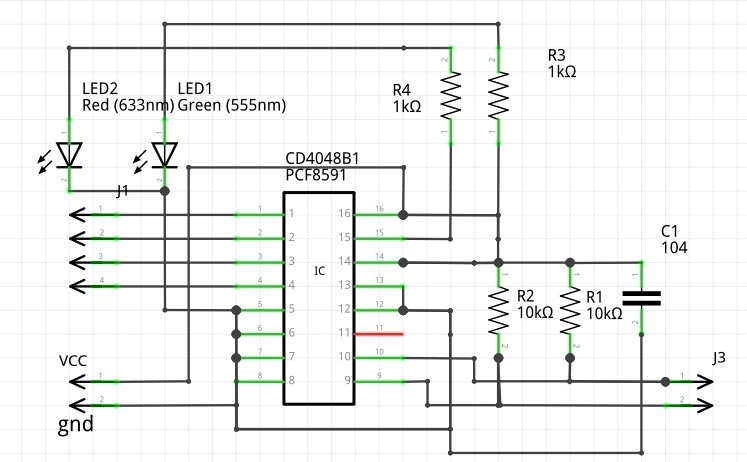
\includegraphics[width=8cm]{figuras/circuito_1.png}
	\caption{Módulo Relé de 8 canais} \label{circuito_1}
\end{figure}


\section{Sensor LDR}

LDR (Light Dependent Resistor), ou fotoresistror, é um dispositivo resistivo que tem a sua resistência alterada de acordo com a quantidade de luz que atinge seus terminais. O componente é feito de um semicondutor de resistência elevada. O sensor apresenta uma alta sensibilidade, com uma resposta rápida as variações de luz e é sensível a todo o espectro visível de luz.[1]

\subsection{Características elétricas}

O LDR apresenta em uma temperatura ambiente uma variação de resistência de aproximadamente 8$\Omega$ até 20K$\Omega$, no escuro total a resistência atinge um valor elevado e 1M$\Omega$. O seu pico de resposta é com o comprimento de onda de 540nm, podendo funcionar dentro de um ambiente com temperaturas variando de -30℃ até 70℃.[Jawaaz Ahmad, 2016]

O sensor aguenta nos seus terminais uma diferença de potencial de até 150 Volts. A leitura do sensor é feita através de um divisor de tensão que é causada pela variação da resistência devido a diferença de iluminação. A tensão lida na saída do divisor de tensão é lida por um conversor AD e assim é transformada em dados para o microcontrolador.[Jawaaz Ahmad, 2016]

\subsection{Princípios físicos de funcionamento}

Um LDR trabalha com a fotocondutividade, que é um efeito ótico onde a condutividade de um material aumenta com a absorção de luz do semicondutor. A exposição à luz do sensor faz com que fótons dessa fonte de luz ao caírem no sensor excitem os elétrons da camada de valência do semicondutor que compõem o sensor. Os elétrons são excitados até adquirirem energia suficiente para chegar a camada de condução do material. Quanto mais elétrons são excitados até a camada de condução do semicondutor, mais corrente passa a fluir pelo semicondutor e assim a resistência que antes era alta, passa a cair com o aumento de luminosidade.[Sunroom Technologies,2008]

\begin{figure}[H]
	\centering
	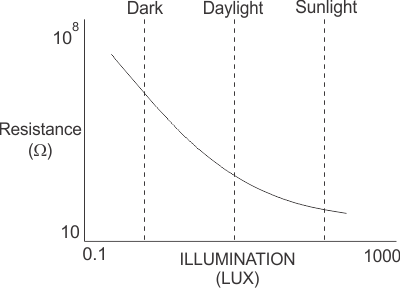
\includegraphics[width=8cm]{figuras/curva_ldr.png}
	\caption{Curva característica de resposta do LDR} \label{curva_ldr}
\end{figure}

\section{Sensores DHT22}

O sensor DHT22 é um sensor digital capacitivo que utiliza uma comunicação serial do tipo Single-bus communication para o envio de dados em 8bits. O sensor apresenta um baixo consumo de potência e uma grande capacidade de envio dos dados eliminando a necessidade de usar amplificadores periféricos para aumentar a potência da saída do sinal. [LIU, 2018]

A tabela \ref{caracteristicas_eletricas} mostra como o sensor deve se comportar sendo alimentado com a voltagem mínima e máxima com que o sensor é capaz de trabalhar. Os valores mínimo, máximo e recomendado para se alimentar o módulo são, respectivamente: 3.3 V, 5.5V e 5V.

\begin{table}[H]
	\centering
	\caption{Características elétricas do sensor LDR}
	\label{caracteristicas_eletricas}
	\begin{tabular}{|l|l|l|l|l|l|}
		\hline
		\textbf{Parameter}                 & \textbf{Condition}                                           & \textbf{min} & \textbf{typ} & \textbf{max} & \textbf{Unit} \\ \hline
		Voltage                            &                                                              & 3.3          & 5            & 5.5          & V             \\ \hline
		\multirow{3}{*}{Power consumption} & Dormancy                                                     & 10           & 15           &              & $\mu$A           \\ \cline{2-6} 
		& Meansuring                                                   &              & 500          &              & $\mu$A           \\ \cline{2-6} 
		& Average                                                      &              & 300          &              & $\mu$A           \\ \hline
		Low level output voltage           & loL{[}5{]}                                                   & 0            &              & 300          & mV            \\ \hline
		High output voltage                & Rp\textless{}25 k$\Omega$                                       & 90\%         &              & 100\%        & VDD           \\ \hline
		Low input voltage                  & Decline                                                      & 0            &              & 30\%         & VDD           \\ \hline
		Input High Voltage                 & Rise                                                         & 70\%         &              & 100\%        & VDD           \\ \hline
		Pull up Resistor                   & \begin{tabular}[c]{@{}l@{}}VDD = 5V\\ VIN = VSS\end{tabular} & 30           & 45           & 60           & k$\Omega$        \\ \hline
		\multirow{2}{*}{Output current}    & turn on                                                      &              & 8            &              & mA            \\ \cline{2-6} 
		& turn off                                                     & 10           & 20           &              & $\mu$A           \\ \hline
		Sampling period                    &                                                              & 2            &              &              & S             \\ \hline
	\end{tabular}

\end{table}


\section{Comunicação}

A comunicação feita através de um único pino de data é feita de acordo com o seguinte protocolo:

\begin{figure}[H]
	\centering
	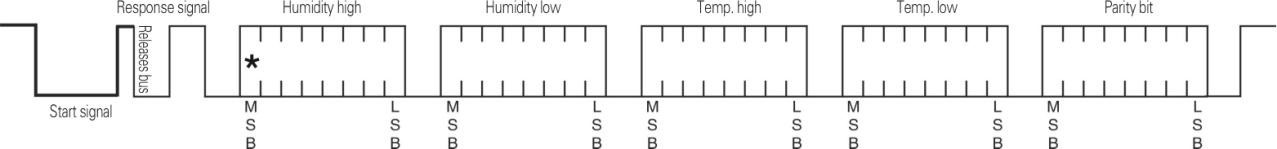
\includegraphics[width=16cm]{figuras/single_bus.jpg}
	\caption{Protocolo de comunicação} 
	\label{single_bus}
\end{figure}

Primeiramente o sensor deve receber um sinal vindo do microcontrolador para que a comunicação seja iniciada, assim é enviado um sinal de resposta pelo sensor estabelecendo assim a comunicação entre o sensor e um microcontrolador. Em seguida são enviados os dados de forma serial seguindo o protocolo da figura 1. Os  dados são enviados em um formato de 40 bits. Os 16 primeiros bits são relacionados aos dados referentes a umidade, os próximos 16 bits se relacionam a temperatura lida pelo sensor e os 8 bits restantes são usados para um controle de paridade do sinal.[LIU, 2018]

A tradução da informação é feita da seguinte forma:

\begin{table}[H]
	\centering
	\caption{My caption}
	\label{my-label}
	\begin{tabular}{|l|l|l|l|l|}
		\hline
		{0000 0010} & {1001 0010} & {0000 0001} & {0000 1101} & {1010 0010} \\ \hline
		High humity 8   & Low humity 8    & High temp. 8    & Low temp. 8     & Parity bit      \\ \hline
	\end{tabular}
\end{table}


Umidade: 0000 0010  1001 0010 = 0292H (Hexadecimal)= 2×256 + 9×16 + 2 = 658    => Humidity = 65.8\%RH

Temperatura: 0000 0001  0000 1101 = 10DH(Hexadecimal) = 1×256 + 0×16 + 13 = 269   => Temp.= 26.9℃ 

Caso a temperatura medida apresente valores negativos, os valores apresentados pelo sensor são precedidos pelo MSB em valor alto conforme o exemplo abaixo:

A temperatura de -10.1 ℃ é expressa como 1 000 0000 0110 0101
Para a conversão utiliza-se a mesma regra anterior desconsiderando que o primeiro bit em nível alto.

0000 0000 0110 0101 = 0065H (Hexadecimal) = 6×16 + 5  = 101  

Então a temperatura é, devido a presença da indicação de sinal negativo do primeiro bit:

=> Temp. = -10.1℃ 

Bit de Paridade: High umidity + Low Humidity + High Temperature + Low Temperature

0000 0010 + 1001 0010 + 0000 0001 + 0000 1101 = 1010 0010

\section{Princípio Físico do Sensor}

A medição de umidade do sensor é feita através de dois eletrodos com um substrato de retenção de umidade entre eles. A mudança de umidade altera a condutividade do substrato e consequentemente a resistência entre os dois eletrodos assim a corrente que passa entre os terminais pode ser lida por um microcontrolador e traduzida em dados legíveis através de um software.[Nedelkovski, 2018]

\begin{figure}[H]
	\centering
	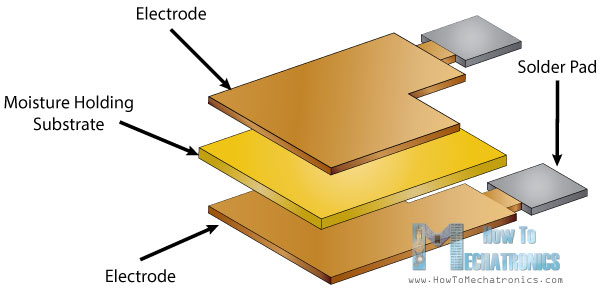
\includegraphics[width=12cm]{figuras/humity_sensor.jpg}
	\caption{Esquema com eletrodos e o substrato de retenção de umidade}
	\label{humity_sensor}
\end{figure}

A realização das medidas de temperatura é feita por um termistor, que é um dispositivo que altera a resistência de acordo com a variação de temperatura.

\begin{figure}[H]
	\centering
	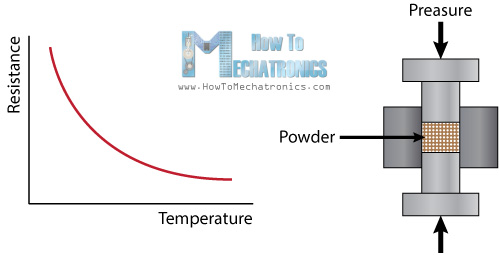
\includegraphics[width=12cm]{figuras/thermistor.jpg}
	\caption{Relação entre temperatura e a resistência do termistor}
	\label{thermistor}
\end{figure}

\section{Motor DC 12V}

Um motor DC é uma máquina elétrica onde a corrente que passa pelos terminais do motor é convertida em força mecânica. A maioria dos motores DC dependem de um campo magnético para realizar essa conversão de energia elétrica em mecânica. A velocidade do motor depende da diferença de potencial entre os terminais, podendo assim ser controlada  através de um ajuste na tensão que chega ao motor.

\subsection{Comunicação}

A comunicação do motor com o microcontrolador é feita através de uma ponte H que permite o controle direcional do motor através da inversão de polaridade que pode ser feita dependendo de como a corrente flui pelo circuito. O funcionamento da ponte H depende da combinação de chaves que permitem ligar e desligar o motor e girar em sentido horário ou anti-horário o eixo do motor.

\subsection{Princípio físico de funcionamento}

Quando um ímã permanente é posicionado em torno de um loop de fio que é ligado a uma fonte de energia D.C., temos os fundamentos de um motor D.C. A fim de fazer o loop de rotação do fio, temos que conectar uma bateria ou fonte de alimentação DC entre suas extremidades, e apoiá-lo para que ele possa girar em torno de seu eixo. Para permitir que o rotor gire sem torcer os fios, as extremidades do loop de arame são conectadas a um conjunto de contatos chamado de comutador, que se esfrega contra um conjunto de condutores chamados de escovas. As escovas fazem contato elétrico com o comutador à medida que ele gira e são conectadas aos cabos positivo e negativo da fonte de energia, permitindo que a eletricidade flua pelo circuito. A eletricidade que flui através do circuito cria um campo magnético que interage com o campo magnético do imã permanente para fazer o laço girar. [Page.M, 1999]

\section{Sonda de pH}

O módulo de sensor pH consiste em captar os íons em solução aquosa e transformar tal informação
em diferença de potencial elétrico em "Volts", tal informação é extraída a partir do bulbo de vidro
projetado na ponta do sensor. A escala de pH é vista de 0 a 14 e mede a concentração em mols a
quantidade de íons. O pH é definido como o logaritmo do inverso da concentração hidrogeniônica
[H+], de uma solução aquosa, em termos matemáticos é descrita como como em situação de
equilíbirio químico:

\begin{figure}[H]
	\centering
	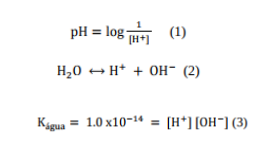
\includegraphics[width=7.5cm]{figuras/calculo_equilibrio.png}
	\caption{Equações matemáticas do pH}
	\label{calculo_equilibrio}
\end{figure}

Desta forma temos que em "água pura"pH = 7,0, ou pH de neutralidade. A escala varia
então de 0,0 (mais ácido) a 14,0 (mais básico). Atualmente, existem pequenos aparelhos portáteis
nomeadoscomo pHmetros que servem como principal indicador deste potencial, que rapidamente
após sua determinação dispõe em um visor um número indicando o valor do pH da solução
utilizada no teste. Basicamente este instrumento utiliza uma sonda chamada eletrodo de vidro, que
ao ser submergida na solução em teste cria uma diferença de potencial elétrico correlacionada com
a concentração hidrogeniônica, permitindo, através do correto tratamento deste sinal de tensão a
medida do valor do pH naquela solução. Cabe lembrar que também há uma certa dependência
desta concentração com a temperatura, por isso a medida do pH deve ser acompanhada pela
medida de temperatura.
As principais aplicações para tal sensor são específicas para meios aquosos, medições da
qualidade da água e aquacultura. 

As principais zonas de padrão de medições estabelecidas no
manual do fornecedor sugerem as seguintes conversões:

\begin{figure}[H]
	\centering
	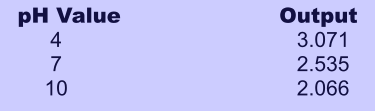
\includegraphics[width=5cm]{figuras/valores_ph.png}
	\caption{Valores de medidas estabelecidas pelo fornecedor de pH e DDP}
	\label{valores_ph}
\end{figure}

\subsection{Especificações gerais}

\begin{itemize}
	\item Tensão máxima de operação 5V
	\item Corrente de trabalho 5-10mA
	\item Escala de detecção pH: 0-14
	\item Escala de detecção em temperatura 0-80 degC
	\item Tempo de resposta menor igual a 5S
	\item Estabilidade de tempo menor igual a 60S
	\item Saída: Analógica
	\item Consumo em funcionamento menor igual a 0,5W
	\item Temperatura de trabalho -10 a +50 deg C
	\item Umidade de trabalho 95 %
	\item Peso 25 g
	\item Dimensão 42mm x 32mm x 20mm
\end{itemize}

\subsection{Documentação}

\begin{figure}[H]
	\centering
	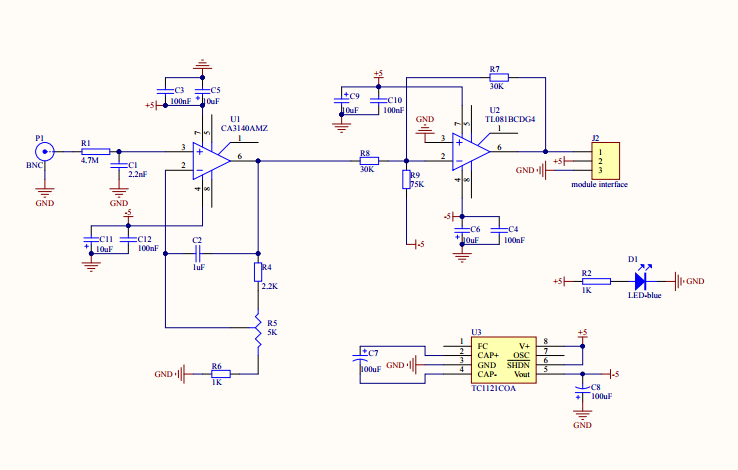
\includegraphics[width=5cm]{figuras/sensor_ph.png}
	\caption{Sensor de pH}
	\label{sensor_ph}
\end{figure}

\begin{figure}[H]
	\centering
	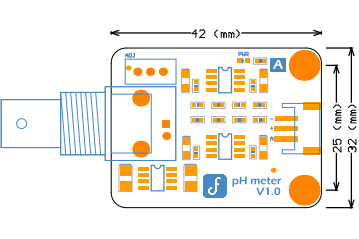
\includegraphics[width=10cm]{figuras/amplificador.png}
	\caption{Amplificador de sinal conexão BNC}
	\label{amplificador}
\end{figure}

\begin{figure}[H]
	\centering
	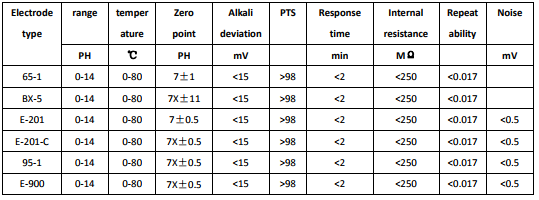
\includegraphics[width=15cm]{figuras/parametros_medicoes.png}
	\caption{Parâmetros de medições de acordo com o tipo de sonda}
	\label{parametros_medicoes}
\end{figure}

\subsection{Esquema de ligação}

\begin{itemize}
	\item 1 x Sonda de pH (conector BNC)
	\item 1 x Placa de circuito do sensor de pH
	\item 1 x Cabo analógico
\end{itemize}

\subsection{Informações de limpeza e manutenção das sondas de pH}

A manutenção e o manuseio têm uma influência significativa sobre a precisão e o tempo de vida
e funcionamento da sonda. Pequenas coisas como bolhas de ar, cristalização, baixo enchimento de
eletrólito. Fuga de KCl ou contaminação podem ter um efeito negativo, sendo importante evitar:

\begin{itemize}
	\item A manutenção e o manuseio têm uma influência significativa sobre a precisão e o tempo de vida
	e funcionamento da sonda. Pequenas coisas como bolhas de ar, cristalização, baixo enchimento de
	eletrólito. Fuga de KCl ou contaminação podem ter um efeito negativo, sendo importante evitar:
	\item Manter a fibra do bulbo hidratada
	\item Evitar bolhas durante a medição
	\item Longos tempos de uso e estabilização
	\item Valores errados e inadequados
	\item Problemas com calibração
\end{itemize}

\section{Sensor de Temperatura para liquídos}

Este sensor de temperatura é a versão a prova de água do sensor DS18B20. Este sensor é indicado
para aplicações onde é necessário medir a temperatura a uma loga distância do microcontrolador
ou em ambientes úmidos. Uma grande vantagem é que por ser digital, a leitura do sensor não sofre
interferência da distância. Por possuir um serial único, vários sensores podem ser interligados na
mesma interface, possibilitando a medição de temperaturas em aplicações de HVAC, máquinas, monitoramento de processos, etc.

Observação do fabricante: Note que a temperatura máxima deste sensor é de 125 ◦ C, mas seu cabo é feito em PVC. Então sugerimos que mantenha o sensor em aplicações abaixo de 100 ◦ C.

\subsection{Especificações gerais}

\begin{itemize}
	\item Tensão de alimentação: 3.0 VDC a 5.5 VDC
	\item Precisão de +/- de -10 ºC a + 85 ºC
	\item Lê temperaturas de a + 125 ◦ C
	\item Resolução de 9 ou 12 bits
	\item Interface 1 fio (1 Wire), ou seja, precisa de somente 1 porta digital
\end{itemize}

\begin{figure}[H]
	\centering
	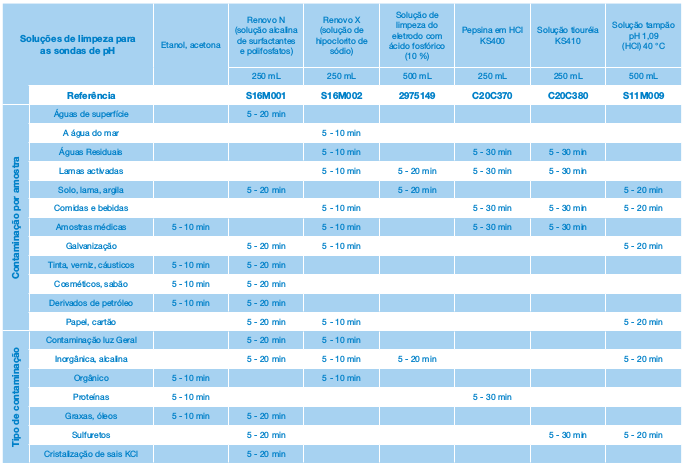
\includegraphics[width=16cm]{figuras/solucoes_especiais.png}
	\caption{Soluções especiais}
	\label{solucoes_especiais}
\end{figure}

